\documentclass[conference]{IEEEtran}
\IEEEoverridecommandlockouts
\usepackage{iftex}
\ifPDFTeX
  \usepackage[T1]{fontenc}
  \usepackage[utf8]{inputenc}
\else
  \usepackage{fontspec}
  \setmainfont{texgyretermes-regular.otf}[
    BoldFont=texgyretermes-bold.otf,
    ItalicFont=texgyretermes-italic.otf,
    BoldItalicFont=texgyretermes-bolditalic.otf]
\fi
\usepackage[spanish,es-tabla]{babel}
\usepackage{cite}
\usepackage{amsmath,amssymb}
\usepackage{graphicx}
\usepackage{booktabs}
\usepackage{url}
\usepackage{etoolbox}
\usepackage{balance}
\usepackage[hidelinks]{hyperref}
\renewcommand{\IEEEkeywordsname}{Palabras clave}
\patchcmd{\abstract}{---}{. }{}{}
\patchcmd{\IEEEkeywords}{---}{. }{}{}

\begin{document}
\title{Aterrizaje lunar con Deep Q-Networks: implementación, análisis de la política y estudio de ablación}
\author{
\IEEEauthorblockN{Thiago Rivas}
\IEEEauthorblockA{C.I. 5.475.680-3 \\
\textit{Facultad de Ingeniería} \\
\textit{Universidad de la República}\\
Montevideo, Uruguay \\
thiago.rivas0021@gmail.com}
\and
\IEEEauthorblockN{Juan Duarte}
\IEEEauthorblockA{C.I. 5.201.302-9 \\
\textit{Facultad de Ingeniería} \\
\textit{Universidad de la República}\\
Montevideo, Uruguay \\
juan.duarte@fing.edu.uy}
\and
\IEEEauthorblockN{Agustin Occhiuzzi}
\IEEEauthorblockA{C.I. 5.480.562-4 \\
\textit{Facultad de Ingeniería} \\
\textit{Universidad de la República}\\
Montevideo, Uruguay \\
agustin.occhiuzzi@fing.edu.uy}
}
\maketitle

\begin{abstract}
Implementamos un agente DQN para LunarLander-v3 y estudiamos su aprendizaje, su política y el efecto de quitar tres componentes del algoritmo. A partir de comparaciones de calibración elegimos una red de dos capas ocultas de 64 unidades y una tasa de aprendizaje de $10^{-3}$. El estudio integrado reúne 32 políticas, ocho por condición, entrenadas durante 300 episodios. El agente completo obtuvo un retorno medio de 137,8 y un 40,44\% de episodios con retorno acumulado de al menos 200, frente a un 0\% del agente aleatorio en la evaluación del notebook. Los cortes del estado muestran decisiones compatibles con frenar la caída y corregir el giro. Al comparar las medias por semilla mediante Mann--Whitney bilateral y corrección de Holm, solo la variante sin replay presentó una diferencia significativa respecto del completo. Las diferencias entre plataformas, la reutilización de escenarios de desarrollo y el número de semillas limitan el alcance de estas conclusiones.
\end{abstract}

\begin{IEEEkeywords}
aprendizaje por refuerzos, DQN, LunarLander, ablación
\end{IEEEkeywords}

\section{Introducción}
En LunarLander-v3 una nave debe aterrizar usando un motor principal y dos laterales. Trabajamos con la versión discreta de Gymnasium~\cite{towers2024}, sin viento. El estado es $s=(x,y,v_x,v_y,\theta,\omega,c_1,c_2)$, con posición, velocidad, ángulo, velocidad angular y dos indicadores de contacto de las patas. Las cuatro acciones son no encender motores, activar el lateral izquierdo, activar el principal o activar el lateral derecho.

Nuestro objetivo fue aprender una política con DQN~\cite{mnih2015} y analizar qué aportan la memoria de repetición, la red objetivo y la exploración. Seguimos el criterio de la tarea: un episodio es exitoso si su retorno acumulado $R=\sum_t r_t$ satisface $R\geq200$, y la tasa de éxito debe ser estrictamente mayor que 10\%. Este umbral por recompensa no equivale a identificar físicamente un aterrizaje.

\section{Solución DQN implementada}
\label{sec:dqn}
La clase \texttt{AgenteDQN} aproxima los valores de acción con una red $Q_\theta$ de entrada de ocho componentes, dos capas ocultas con ReLU y cuatro salidas lineales. Cada salida estima el retorno futuro descontado de una acción~\cite{sutton2018}. La red de referencia tiene 4996 parámetros. A diferencia del DQN aplicado a imágenes de Atari~\cite{mnih2015}, usamos directamente el vector de estado y una red completamente conectada. No normalizamos las observaciones ni recortamos las recompensas.

Guardamos las transiciones $(s,a,r,s',d)$ en una memoria de repetición (\textit{replay}) de capacidad fija. En cada actualización extraemos un minilote uniforme sin reemplazo. Esto permite reutilizar experiencias y reduce la dependencia inmediata entre transiciones consecutivas. Una segunda red $Q_{\theta^-}$, inicialmente igual a $Q_\theta$, permanece sin gradientes y se actualiza mediante copias periódicas. Para cada transición calculamos
\begin{equation}
 z=r+\gamma(1-d)\max_{a'}Q_{\theta^-}(s',a').
\end{equation}
Minimizamos la pérdida SmoothL1, equivalente a Huber con $\beta=1$, entre $Q_\theta(s,a)$ y $z$, promediada sobre el minilote. El objetivo se calcula fuera del grafo de gradientes. Usamos Adam y limitamos la norma del gradiente para moderar actualizaciones grandes.

La variable $d$ corresponde a \texttt{terminated}. Un truncamiento por tiempo detiene el episodio, pero conserva el término de valor futuro del estado siguiente. Esta distinción evita tratar el límite de 1000 pasos como un estado terminal del problema. En entrenamiento elegimos una acción aleatoria con probabilidad $\varepsilon$ y una acción de máximo valor en los demás casos. Tras $e$ episodios completos usamos
\begin{equation}
 \varepsilon_e=\max\left(0{,}05,\ 1-0{,}95\frac{e}{200}\right).
\end{equation}
En evaluación usamos siempre $\arg\max_a Q_\theta(s,a)$, sin explorar ni actualizar los pesos.

\begin{table}[t]
\caption{Configuración de referencia A0}
\label{tab:hiper}
\centering
\begin{tabular}{@{}ll@{}}
\toprule
Parámetro & Valor \\
\midrule
Red Q & $8\to64\to64\to4$, ReLU \\
Adam & $\eta=10^{-3}$, $\beta_1=0{,}9$, $\beta_2=0{,}999$ \\
Descuento & $\gamma=0{,}99$ \\
Memoria / minilote & 50\,000 / 64 transiciones \\
Inicio / frecuencia & 1000 pasos / cada 4 pasos \\
Copia a red objetivo & Cada 1000 pasos de entorno \\
Exploración & Lineal por episodio, $1\to0{,}05$ \\
Pérdida / gradiente & Huber ($\beta=1$) / norma $\leq10$ \\
Presupuesto & 300 episodios, hasta 1000 pasos \\
\bottomrule
\end{tabular}
\end{table}

La tabla~\ref{tab:hiper} resume la configuración. Adam usa además $\epsilon=10^{-8}$ y no aplica regularización por decaimiento de pesos. La primera actualización ocurre en el paso 1000. Cuando coincide con una copia a la red objetivo, primero actualizamos la red que aprende. El presupuesto se cumple sin parada anticipada y evaluamos los pesos finales, sin elegir el mejor episodio a posteriori.

\section{Selección de hiperparámetros}
\label{sec:calibracion}
La calibración tuvo tres líneas de trabajo: arquitectura y tasa de aprendizaje, capacidad de replay y esquema de exploración. Los pilotos cortos permitieron comprobar la implementación. Para decidir la referencia usamos las comparaciones guardadas, cuyos presupuestos y configuraciones no fueron siempre iguales.

En la comparación de arquitectura y tasa entrenamos A0, A1 y A2 con las semillas 42 y 1042, durante 300 episodios, y evaluamos cada política en 200 escenarios. A1 cambia simultáneamente el ancho de las capas y la tasa respecto de A0. Agregamos A2 para separar esos factores: A0 frente a A2 cambia solo la tasa configurada, y A2 frente a A1 cambia solo el ancho. Después probamos A3, con la misma arquitectura de A0 y una tasa mayor. La tabla~\ref{tab:calibracion} muestra los retornos calculados a partir de los CSV originales.

\begin{table}[t]
\caption{Calibración de arquitectura y tasa: retorno medio de 200 episodios por política}
\label{tab:calibracion}
\centering
\begin{tabular}{@{}lcrrr@{}}
\toprule
Config. & Capas ocultas & $\eta$ & Semilla 42 & Semilla 1042 \\
\midrule
A0 & 64, 64 & $10^{-3}$ & 167,2 & 209,8 \\
A1 & 128, 128 & $5\cdot10^{-4}$ & 142,1 & 33,7 \\
A2 & 64, 64 & $5\cdot10^{-4}$ & $-7{,}4$ & 7,7 \\
A3 & 64, 64 & $5\cdot10^{-3}$ & 203,3 & 99,9 \\
\bottomrule
\end{tabular}
\end{table}

A0 obtuvo una media entre las dos semillas de 188,5, frente a 87,9 de A1, 0,1 de A2 y 151,6 de A3. Elegimos A0 como referencia para el estudio integrado. Esta evidencia favorece esa elección dentro de las pruebas realizadas, pero A3 supera a A0 en la semilla 42. Dos entrenamientos por configuración no permiten afirmar optimalidad ni superioridad general. Tampoco atribuimos los tiempos de ejecución únicamente al tamaño de la red, porque cambian los pasos efectivos y la carga de la máquina.

En el ensayo histórico de replay comparamos capacidades de 100\,000 y 10\,000 transiciones, junto con un prototipo sin replay. Con semilla 42, 500 episodios de entrenamiento y 50 de evaluación, los retornos medios fueron 247,7, 223,6 y $-87{,}7$, respectivamente. Las tasas de éxito fueron 86\%, 80\% y 0\%. Ese agente usaba capas de 128 unidades y $\eta=5\cdot10^{-4}$. Fue una comparación de capacidad, no de tamaños de minilote. La capacidad final de 50\,000 y el minilote de 64 pertenecen a la referencia A0, sin una búsqueda controlada que pruebe que sean los mejores valores.

El ensayo histórico de exploración usó cinco semillas, 600 episodios de entrenamiento y 100 de evaluación por política. Con una red 128/128, actualización suave de la red objetivo y $\varepsilon$ mínimo de 0,01, el decaimiento exponencial por episodios obtuvo 177,1 de retorno medio y el lineal en 50\,000 pasos obtuvo 127,1. El contraste bilateral de Mann--Whitney registrado dio $p=0{,}2222$, sin ajuste por comparaciones múltiples. La tendencia no prueba superioridad del esquema exponencial. Además, el esquema lineal por episodios del estudio final es distinto de ambos. Conservamos el esquema de A0 para la comparación común, sin presentar aquellos resultados como una validación directa de esta decisión. Estos antecedentes están separados de las 32 políticas finales.

\section{Aprendizaje y desempeño final}
\label{sec:resultados}
\subsection{Selección y evaluación}
El manifiesto integrado selecciona ocho políticas completas y ocho sin replay de Fran, ocho sin red objetivo de Thiago y ocho sin exploración de Agustín. Las tres políticas completas adicionales de Thiago quedan fuera de los promedios y tests. La selección se basa en procedencia y cobertura de semillas, no en rendimiento.

Las semillas de entrenamiento son 42, 1042, 2042, 3042, 4042, 5042, 6042 y 7042. Fijamos los generadores de Python, NumPy, PyTorch y del espacio de acciones. El episodio $i$, contado desde cero, reinicia el entorno con la semilla de entrenamiento más $i$. Cada política final se evalúa sin exploración sobre las semillas 10000 a 10199. Son escenarios de desarrollo, ya utilizados durante la calibración. La evaluación reservada de 30000 a 30199 no se realizó.

La unidad experimental es una política entrenada. Los 200 episodios estiman el desempeño de esa política y no son 200 entrenamientos independientes. En la tabla~\ref{tab:resultados}, cada celda es la media de esos 200 retornos. La última parte resume las ocho medias con igual peso y su desviación estándar muestral (DE). La tasa de éxito promedia las ocho proporciones, lo que aquí equivale a sumar los éxitos sobre 1600 episodios, porque todas las políticas tienen el mismo número de evaluaciones.

\begin{table}[t]
\caption{Evaluación original del estudio integrado por semilla de entrenamiento}
\label{tab:resultados}
\centering
\begin{tabular}{@{}lrrrr@{}}
\toprule
Semilla & Completo & Sin objetivo & Sin replay & Sin explor. \\
\midrule
42   & 174,9 & 140,3 & $-28{,}2$ & $-168{,}7$ \\
1042 & 183,2 & $-211{,}9$ & 122,8 & 62,6 \\
2042 & 80,6  & 189,3 & 6,2 & 150,7 \\
3042 & 69,5  & 20,6 & $-129{,}5$ & $-70{,}2$ \\
4042 & 60,5  & 0,7 & $-129{,}2$ & $-133{,}3$ \\
5042 & 121,9 & 81,7 & 107,6 & 65,9 \\
6042 & 203,2 & 149,7 & 38,3 & 119,2 \\
7042 & 208,7 & 7,0 & 5,1 & 180,3 \\
\midrule
Media & 137,8 & 47,2 & $-0{,}8$ & 25,8 \\
DE entre semillas & 62,0 & 126,6 & 94,5 & 132,8 \\
Éxitos / 1600 & 647 & 352 & 189 & 287 \\
Éxito (\%) & 40,44 & 22,00 & 11,81 & 17,94 \\
\bottomrule
\end{tabular}
\end{table}

\subsection{Curvas y comparación con el azar}
La figura~\ref{fig:curvas} muestra una mejora del completo: el retorno promedio de sus primeros 20 episodios es $-177{,}6$ y el de los últimos 20 es 147,0. Las curvas de las ablaciones también mejoran respecto del inicio, pero no mantienen el mismo nivel. Sin red objetivo aparece una dispersión amplia al final. Estas observaciones describen el entrenamiento, que todavía incluye exploración, y no sustituyen los contrastes sobre la evaluación final.

\begin{figure}[t]
\centering
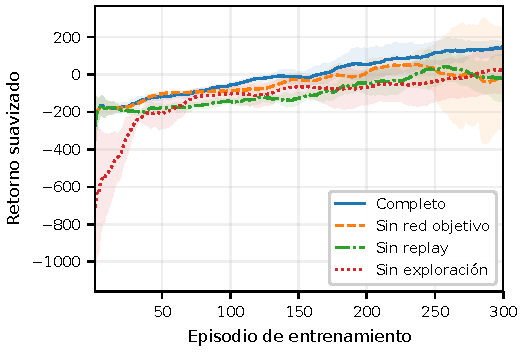
\includegraphics[width=\columnwidth]{figuras/curvas_aprendizaje.pdf}
\caption{Retorno de entrenamiento suavizado con una media móvil causal de hasta 20 episodios. Cada línea promedia ocho semillas. Las bandas son $\pm1$ DE muestral entre las curvas suavizadas, no intervalos de confianza.}
\label{fig:curvas}
\end{figure}

El completo obtuvo 647 éxitos en 1600 evaluaciones (40,44\%). Siete de las ocho políticas superan estrictamente el 10\%. La excepción es la semilla 3042, con 7/200 éxitos (3,5\%). El rango de las tasas individuales va de 3,5\% a 71,5\%, por lo que cumplir el criterio en promedio no garantiza cumplirlo en cada entrenamiento.

Para comparar con el azar en una misma plataforma usamos la salida ejecutada del notebook integrado. Allí se reevaluó el completo de semilla 42 en 200 episodios y obtuvo $168{,}86\pm81{,}11$ de retorno y 63/200 éxitos (31,5\%). El agente aleatorio, con el generador de acciones fijado en 42 y los mismos escenarios, obtuvo $-183{,}17\pm111{,}96$ y 0/200 éxitos. En estos dos valores, $\pm$ indica la desviación estándar de los 200 retornos con divisor 200, no dispersión entre entrenamientos. Es una comparación descriptiva de una política con el azar. Esta reevaluación local no coincide exactamente con la evaluación original de esa red (174,90 y 68/200), por lo que no la usamos para reemplazar datos del estudio.

\section{Análisis de la política}
\label{sec:politica}
Analizamos los pesos finales mediante tres cortes de $101\times101$ puntos. El estado de referencia tiene $x=v_x=\theta=\omega=c_1=c_2=0$, $y=0{,}8$ y $v_y=-0{,}3$. Variamos dos dimensiones por vez: $(x,v_x)$, $(\theta,\omega)$ y $(y,v_y)$. Las otras seis permanecen fijas. Elegimos la semilla 42 por ser la primera del protocolo, sin seleccionarla por desempeño. La figura~\ref{fig:cortes} presenta la acción greedy y el mayor valor Q, calculados directamente con los pesos guardados.

\begin{figure*}[t]
\centering
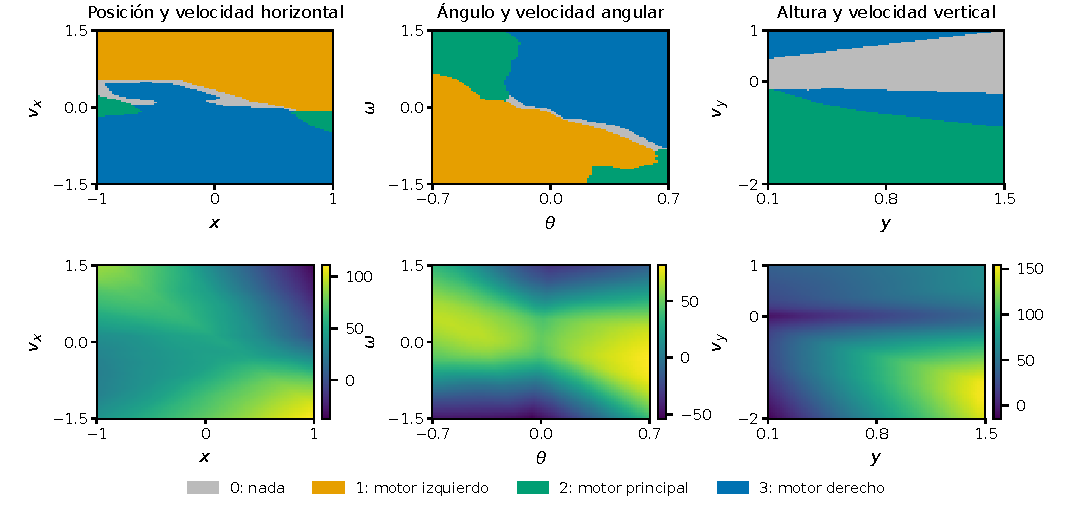
\includegraphics[width=\textwidth]{figuras/cortes_politica.pdf}
\caption{DQN completo, semilla 42. Arriba: acción greedy en cada estado sintético. Abajo: mayor valor $Q_\theta(s,a)$ entre las cuatro acciones, con escala propia por panel. En cada columna solo varían las dos dimensiones de los ejes. Las demás toman los valores del estado de referencia descrito en el texto. Las regiones no representan frecuencias de visita ni probabilidades de éxito.}
\label{fig:cortes}
\end{figure*}

En el corte vertical aparece una frontera inclinada: el motor principal se activa para velocidades descendentes de mayor magnitud, y cerca del suelo se activa con caídas más lentas. Esto es compatible con frenar según la altura disponible. Por encima de esa región aparecen tanto la inacción como el motor lateral derecho, por lo que el corte no se reduce a una regla binaria de frenado.

En el plano angular predominan motores laterales opuestos a ambos lados de una frontera que depende de $\theta$ y $\omega$. Cerca de esa frontera, el motor derecho reduce el ángulo y el izquierdo lo aumenta. La forma es compatible con corregir conjuntamente inclinación y giro. No demuestra que la red implemente un controlador lineal en todo el espacio. En los cortes de las ocho semillas conservados en el notebook observamos la misma organización general, aunque cambian las fronteras y las zonas de inacción y motor principal.

En el plano horizontal, una velocidad positiva suficientemente alta favorece el motor izquierdo, compatible con reducir la deriva hacia la derecha. La división depende también de $x$ y es asimétrica. No podemos inferir una preferencia global por un lado a partir de este único estado de referencia. Los valores Q estiman retorno descontado, no una probabilidad de aterrizar ni el retorno acumulado de un episodio. Las zonas con Q alto y caída muy rápida ilustran por qué una predicción de la red, por sí sola, no valida una acción.

Los cortes usan estados sintéticos, algunos posiblemente poco visitados o inalcanzables. Las figuras originales de análisis superponen proyecciones de estados de 20 episodios reales. Esos puntos permiten ubicar regiones visitadas en cada plano, pero sus otras seis coordenadas generalmente difieren de las fijadas en el corte. Por eso tampoco validan por sí solos las decisiones mostradas para esos estados sintéticos.

Para estudiar los finales de episodio usamos la reevaluación auxiliar local de las 32 redes en \texttt{policy\_all}, con 20 escenarios por red (10000 a 10019). La tabla~\ref{tab:fines} se calcula con esos registros, separados de los CSV del estudio y de los análisis históricos de 24 redes. Clasificamos como posado el final con \texttt{terminated} y recompensa del último paso $+100$. Las demás terminaciones se agrupan como choque o salida, y los truncamientos corresponden al límite temporal.

\begin{table}[t]
\caption{Finales de episodio en la reevaluación auxiliar macOS: 160 episodios por condición}
\label{tab:fines}
\centering
\begin{tabular}{@{}lrrr@{}}
\toprule
Condición & Posado & Choque/salida & Truncado \\
\midrule
Completo & 105 & 7 & 48 \\
Sin red objetivo & 66 & 54 & 40 \\
Sin replay & 22 & 135 & 3 \\
Sin exploración & 35 & 48 & 77 \\
\bottomrule
\end{tabular}
\end{table}

En el completo predominan los truncamientos entre los episodios que no terminan posados (48 de 55), mientras que sin replay predominan los choques o salidas (135 de 160). Estos conteos ayudan a describir el comportamiento, pero no son tasas de éxito por recompensa. Por ejemplo, el completo tiene 105 finales posados y solo 68 episodios con $R\geq200$ en esta reevaluación. Un aterrizaje con mucho gasto de combustible puede no alcanzar el umbral.

\section{Estudio de ablación}
\label{sec:ablacion}
\subsection{Variantes y test estadístico}
Quitamos un componente por condición. Sin red objetivo, el valor futuro se calcula con la propia red que aprende, también sin propagar gradientes a través del objetivo. Sin replay, usamos solo la transición actual en los pasos programados de actualización, con minilote efectivo de uno. Conservamos el inicio en 1000 pasos y la frecuencia de cuatro pasos, de modo que las transiciones intermedias no se reutilizan. Sin exploración, fijamos $\varepsilon=0$ desde el inicio. La aleatoriedad de la inicialización y del entorno permanece.

Usamos como test principal U de Mann--Whitney bilateral exacto~\cite{mann1947}, sobre las ocho medias de evaluación de cada condición. No exige normalidad y contrasta igualdad de distribuciones. No es, en general, un test exclusivo de diferencia de medias o medianas. Corregimos los tres contrastes contra el completo mediante Holm~\cite{holm1979}, con nivel familiar $\alpha=0{,}05$. Verificamos que no hubiera empates entre las medias utilizadas. La prueba supone independencia de las muestras, una condición que debe tomarse con cautela por el uso de semillas comunes entre variantes.

\begin{table}[t]
\caption{Contrastes contra el completo, ocho políticas por condición}
\label{tab:tests}
\centering
\begin{tabular}{@{}lrrrrr@{}}
\toprule
Ablación & $\Delta$ & U & $p$ MW & $p$ Holm & $p$ W/H \\
\midrule
Sin objetivo & 90,6 & 47 & 0,1304 & 0,1304 & 0,1094 \\
Sin replay & 138,7 & 57 & 0,0070 & 0,0210 & 0,0234 \\
Sin explor. & 112,0 & 50 & 0,0650 & 0,1299 & 0,0781 \\
\bottomrule
\end{tabular}
\smallskip
\parbox{\columnwidth}{\footnotesize $\Delta$: retorno medio del completo menos el de la ablación. U corresponde al completo. W/H: Wilcoxon emparejado, con Holm aplicado a sus tres contrastes como familia de sensibilidad.}
\end{table}

La tabla~\ref{tab:tests} muestra que solo la variante sin replay difiere significativamente del completo con el criterio principal. El completo tiene mayor media en las ocho semillas emparejadas y supera a la ablación en 57 de los 64 pares posibles entre políticas ($\mathrm{U}/64=0{,}891$). La diferencia media es 138,7 puntos. Esto respalda la utilidad de replay en la configuración estudiada, teniendo presente que la ablación también cambia el tamaño efectivo del minilote y la reutilización de transiciones.

Sin red objetivo y sin exploración presentan medias menores, pero sus $p$ ajustados son 0,1304 y 0,1299. No rechazamos la hipótesis nula con este diseño. Esto no demuestra equivalencia ni que esos componentes sean innecesarios. Con ocho semillas y alta dispersión, las diferencias descriptivas de 90,6 y 112,0 puntos no bastan para sostener una conclusión de superioridad estadística.

Como sensibilidad aplicamos Wilcoxon bilateral de rangos con signo~\cite{wilcoxon1945}, emparejando las medias por número de semilla. El método requiere pares con sentido experimental, independencia entre pares y simetría de la distribución de sus diferencias. No hubo diferencias nulas ni empates en sus magnitudes, pero con ocho pares no podemos dar por comprobada la simetría. Sin exploración da $p=0{,}0391$ antes del ajuste y $p=0{,}0781$ después de Holm. Solo sin replay sigue siendo significativo. No cambiamos el test principal para aprovechar un $p$ sin ajustar. El emparejamiento por semilla tampoco garantiza trayectorias comparables entre equipos.

\balance
\subsection{Plataformas y código}
Las condiciones completa y sin replay se entrenaron en Windows 11 AMD64, con Python 3.12.10, PyTorch 2.15.0+cpu y NumPy 2.5.3. Sin exploración se entrenó en otro entorno Windows 11 AMD64, con Python 3.12.9, PyTorch 2.14.1+cpu y NumPy 2.5.4. Sin red objetivo usó macOS ARM64, Python 3.12.16, PyTorch 2.14.1 y NumPy 2.5.4. Todas registran Gymnasium 1.4.0, Box2D 2.3.10 y ejecución en CPU con un hilo de cómputo de PyTorch. Los hilos de interoperación fueron 10, 4 y 8, respectivamente.

Los metadatos registran distintas revisiones Git: \texttt{f3f0184} y \texttt{148db4f} para el completo, \texttt{f3f0184} sin replay, \texttt{0686cbf} sin exploración y \texttt{5bf74d4} sin red objetivo. Al contrastar esas revisiones verificamos que el notebook de entrenamiento contiene el mismo código. Sus dos hashes registrados corresponden a saltos de línea LF y CRLF. Esto evita atribuir una diferencia algorítmica a la mera diferencia de hash, pero no elimina las diferencias del entorno de ejecución. Como no cruzamos todas las condiciones en todas las plataformas, los tests no separan el efecto del componente quitado de esos posibles factores de confusión.

\section{Limitaciones}
El presupuesto común es de episodios, no de interacciones ni actualizaciones. Las corridas consumieron entre 32\,968 y 241\,521 pasos, según la duración de sus trayectorias. Por eso comparamos resultados al cabo de 300 episodios, sin afirmar convergencia ni igual costo computacional. Ocho semillas ofrecen una descripción todavía limitada de la variabilidad del entrenamiento.

La reutilización de escenarios de desarrollo puede favorecer las decisiones tomadas durante la calibración. Al no haberse ejecutado la evaluación reservada, las cifras no estiman desempeño sobre un conjunto completamente independiente de ese proceso. Las reevaluaciones auxiliares sirven para analizar políticas guardadas, no agregan réplicas de entrenamiento. Finalmente, los cortes cubren solo tres planos con seis coordenadas fijas, y las conclusiones sobre replay corresponden a la ablación concreta de transición actual y minilote uno.

\section{Conclusiones}
Implementamos una solución DQN que supera el criterio de éxito de la tarea en el promedio del estudio y en siete de sus ocho políticas completas. La evaluación local del notebook también muestra una mejora clara respecto del agente aleatorio. Los cortes permiten reconocer decisiones de frenado y corrección angular, junto con asimetrías y variación entre semillas.

La evidencia estadística más firme del estudio corresponde a replay: quitarlo reduce el desempeño y produce una diferencia significativa tras corregir los tres contrastes. Los resultados de red objetivo y exploración quedan inconclusos con estas corridas. Para precisar esos efectos sería necesario ampliar las semillas y repetir las condiciones en entornos comparables, además de realizar la evaluación reservada una vez cerradas las decisiones.

\section*{Uso de Inteligencia Artificial}
Usamos herramientas de IA como apoyo para desarrollar y revisar código, organizar y contrastar resultados, y redactar y editar este informe. La asistencia incluyó la escritura de la prosa y la preparación del LaTeX. Las cifras se contrastaron con el código, las configuraciones, los manifiestos y las salidas guardadas. Durante la preparación del informe no reentrenamos agentes ni reemplazamos resultados originales.

\begin{thebibliography}{00}
\bibitem{towers2024} M.~Towers \textit{et al.}, ``Gymnasium: A standard interface for reinforcement learning environments,'' arXiv:2407.17032, 2024.
\bibitem{mnih2015} V.~Mnih \textit{et al.}, ``Human-level control through deep reinforcement learning,'' \textit{Nature}, vol.~518, pp.~529--533, 2015, doi:~10.1038/nature14236.
\bibitem{sutton2018} R.~S.~Sutton y A.~G.~Barto, \textit{Reinforcement Learning: An Introduction}, 2.\textsuperscript{a} ed. MIT Press, 2018.
\bibitem{mann1947} H.~B.~Mann y D.~R.~Whitney, ``On a test of whether one of two random variables is stochastically larger than the other,'' \textit{Ann. Math. Statist.}, vol.~18, no.~1, pp.~50--60, 1947.
\bibitem{holm1979} S.~Holm, ``A simple sequentially rejective multiple test procedure,'' \textit{Scand. J. Statist.}, vol.~6, no.~2, pp.~65--70, 1979.
\bibitem{wilcoxon1945} F.~Wilcoxon, ``Individual comparisons by ranking methods,'' \textit{Biometrics Bulletin}, vol.~1, no.~6, pp.~80--83, 1945.
\end{thebibliography}
\end{document}
